\documentclass[12pt]{article}
\usepackage{geometry}
\geometry{a4paper, total={170mm,257mm},left=20mm, top=20mm, }
\usepackage[colorlinks=true,linkcolor=blue,urlcolor=black]{hyperref}
\usepackage{bookmark}
\usepackage[autostyle, english = american]{csquotes}
\usepackage{appendix}
\usepackage{graphicx}
\begin{document}
\begin{titlepage}
\centering
\vfill
\vspace*{4\baselineskip}
{\bfseries\Large
Labtainers Instructor Guide\par
}
\vspace*{4\baselineskip}
{\bfseries
Fully provisioned cybersecurity labs\par
}
\vspace*{2\baselineskip}
\today
\vfill
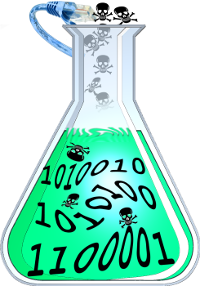
\includegraphics[width=2in]{labtainer5-sm.png}
%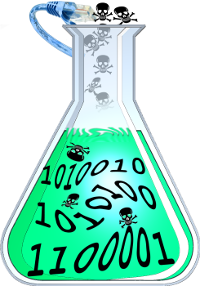
\includegraphics[width=\linewidth, scale=0.50,natwidth=200, natheight=286]{labtainer5-sm.png}
\vfill
\end{titlepage}

\section {Introduction}
This manual is intended for use by instructors who assign and/or grade
labs using Labtainers.
Labtainers assume you have a Linux system, e.g., a virtual machine (VM).  
The easiest path is to use our pre-built VM available at the Labtainer
website \url{https://my.nps.edu/web/c3o/virtual-machine-images}.
Alternately, refer to
in Appendix A of the \underline{Labtainer Student Guide} for installation of VirtualBox 
and a Linux system.
Note that any Linux system can be used as long as it supports Docker.
If Labtainers is to be used on a Linux system other than the pre-built VM,
refer to the \underline{Labtainer Student Guide} for information on
installing Labtainers.

Labtainers provide a consistent execution environment for performing
laboratory exercises, and can include execution of several different
computers interconnected via virtual networks.  Refer to our published
papers at \url{https://my.nps.edu/web/c3o/labtainers} for additional information
on the use of Labtainers.  And see the \underline{Lab Designer User Guide}"
at \url{https://my.nps.edu/documents/107523844/109121513/labdesigner.pdf} for 
information on creating and maintaining Labtainer exercises.

\subsection{Assigning a Lab}
Student instructions for using Labtainers are in the \underline{Labtainer Student Guide}.  
Students work from the {\tt labtainer-student} directory, i.e.,
\begin{verbatim}
    cd ~/labtainer/trunk/scripts/labtainer-student
\end{verbatim}
Available labs are listed via the {\tt labtainer} script:
\begin{verbatim}
    labtainer
\end{verbatim}
\noindent Start a lab by providing its name as an argument to the {\tt labtainer} command.
This will typically display a link to a lab manual, or will display a lab manual in one of
the resulting virtual terminals.  You can interact with the resulting computers just as a
student would.

\subsection{Assessing a Lab}
When the student stops a lab, i.e., using {\tt stoplab}, Labtainers creates a zip file of
student artifacts (including lab reports) and then displays the path to this zip file to
the student.  The easiest way for the student to forward this zip file to you is by starting
a browser on the Linux VM and either emailing you the zip file, or uploading the file
into an LMS, (e.g., Sakai).  Alternately, the student can define a shared folder in the VM
and copy the zip to the host computer.

Collect all of the lab zip files from each student into your Labtainer transfer directory, which
is typically at
\begin{verbatim}
    ~/labtainer_xfer/<labname>
\end{verbatim}
\noindent where labname is the name of the lab.  Do not unzip the files.  Alternately student
assignments can be bulk-collected from a learning management system (LMS) per Appendix \ref{lms collection}
and the resulting zip  would be copied into the
Labtainer transfer directory.  Again, do not unzip files and do not change the file names of zip files.

Instructor assessment of labs takes place from the {\tt labtainer-instructor} directory, i.e.,
\begin{verbatim}
    cd ~/labtainer/trunk/scripts/labtainer-instructor
\end{verbatim}

\noindent Use the {\tt gradelab} command to assess results for a given lab:
\begin{verbatim}
    gradelab <labname>
\end{verbatim}
\noindent A table of lab results with one row per student and
a column for each goal will be displayed.  A description of the goals follows the table.
Note that not all labs include automated assessment.  For those labs, you will see this
message:
\begin{verbatim}
  No automated assessment for this lab
\end{verbatim}
\noindent Even when no automated assessment is performed, you can still observe student performance
artifacts, e.g., the {\tt .bash\_history} file as described below in \ref{review-artifacts}.

Use the {\tt -r} option to get perform a fresh grading, e.g., if you've removed files from the {\tt labtainer\_xfer} directory.
Use the {\tt -u } option to update your gradelab container.  This may be necessary if it reports errors.

Student reports (if any) are  copied into 
\begin{verbatim}
    ~/labtainer_xfer/<labname>/docs
\end{verbatim}
\noindent on the Linux host.  If LMS assignment collection is used, then student reports should
be looked for in 
\begin{verbatim}
    ~/labtainer_xfer/<labname>/reports
\end{verbatim}
\noindent which also includes reports separately uploaded into the LMS.

\subsubsection{Review artifact details}
\label{review-artifacts}
You can view all student results, including their original artifacts by using the {\tt -d} flag
with the {\tt gradelab} command.  This results in a virtual terminal connected to a grading
container that contains all student artifacts and results.  If you have not first run the
{\tt gradelab} command without the ``-d'' option, run {\tt instructor.py} from within the
virtual terminal to cause the zip files to be extracted.  A student's home directory can
then be found in
\begin{verbatim}
<student email>/<lab>.<container>.student
\end{verbatim}
\noindent There you will find the {\tt .bash\_history} file along with the student-created files.
Student artifacts collected by the framework are found in 
\begin{verbatim}
<student email>/<lab>.<container>.student/.local/result
\end{verbatim}

\noindent The {\tt -d} option is also used when debugging automated assessment configuration
files.  You can create additional virtual terminals into the grading container by reissuing
the gradelab command with the {\tt -a} flag.  When you are finished, or wish to stop working, type:
\begin{verbatim}
    stopgrade
\end{verbatim}

\section{Managing Labtainer Installations and Updates}
Any given Labtainers installation can be brought up to date to the latest version by using the
\begin{verbatim}
   update-labtainer.sh
\end{verbatim}
\noindent command from the {\tt labtainer-student} directory.  The current version of a Labtainer installation is seen by using:
\begin{verbatim}
   labtainer -v
\end{verbatim}
\noindent
The first time any given lab exercise is started, the latest version of that lab is automatically pulled from
the Docker Hub registry.
Note however that any given lab is not updated by the {\tt update-labtainer.sh} command once the lab has been started.  
To update a specific lab to the latest version after it has been started the previous version of that lab must be deleted
using:
\begin{verbatim}
   removelab.py <labname>
\end{verbatim}
\noindent The next time the lab is started, the latest version will be retrieved from the Docker registry.

\noindent \\If you want to update the labtainer.grader docker image (and delete the previous image and grader containers) use:
\begin{verbatim}
   gradelab -u <labname>
\end{verbatim}


\subsection{Suggestions for student workflow}
A student's work on any given lab is preserved until and unless the student restarts the lab using the ``-r'' 
option on the {\tt labtainer <labname> -r} command.  When taking a break from work on a lab, the student can
either stop the lab using {\tt stoplab}, or simply pause the VM.  However, if the student wishes to perform other
Labtainer-related work on the VM, (e.g., revisit a previous lab), they should first use {\tt stoplab} for the current
lab.  When they restart the lab, none of their work will be lost.

\subsection{Deploying without the Internet}
Labtainers pulls Docker images from Docker Hub when a student first runs any given lab.  You can deploy
Labtainers within environments that have no Internet connection by first creating your own 
VM template.  Start with the standard Labtainers VM, and run the script at 
\begin{verbatim}
   $LABTAINER_HOME/setup_scripts/pull_lab.py
\end{verbatim}
\noindent to pull images for your desired labs onto the VM.  Then replicate that VM for each user, e.g., by
exporting it as an appliance.

\subsection{Deploying on servers}
Labtainer VMs can run on servers that students access via web browsers using tools such as VMWare Horizon 
and Apache Guacamole. In these environments, each student is allocated a VM, and that VM's desktop is seen 
by the student in the browser.  Students deliver their results to instructors by starting a browser
within the VM, e.g., to access an LMS or web-mail account.

\section{Customizing Labtainers}
Creating new labs and modifying existing labs is described in the \textit{Labtainers Lab Designer User Guide}.
\url{https://nps.box.com/shared/static/12n0y4yue49xcxtpv0jybgqiiskx8pr6.pdf}

That guide also describes how to provide your students with custom versions of the lab manuals, and how to
publish new labs so that they can be incorporated into your student's Labtainers instances, and shared
with other educators.

\newpage
\appendix
\section{\\LMS Assignment Collection}
\label{lms collection}
\subsection{Sakai}
In the Sakai Assignments section, select the ``In / New'' entry for the appropriate assignment.
The resulting page should enumerate each student who has submitted an assignment.  In the upper right,
click the ``Download All'' link, and then click the ``Student submission attachment(s)'' option and
click the ``Download'' button.  Copy the resulting zip into the lab transfer directory 
on the Linux host, i.e.,
\begin{verbatim}
    ~/labtainer_xfer/<labname>
\end{verbatim}
\noindent Do not unzip the file and do not change its file name.
You can then run the {\tt gradelab <labname>} command from the {\tt labtainer-instructor} directory.
In addition to the assessment summary, any student lab reports will be available in:
\begin{verbatim}
   ~/labtainer_xfer/<labname>/reports/<student name> 
\end{verbatim}
\noindent Those reports will include any that the student separately uploaded into Sakai (it is 
important to remind students to NOT change the name of lab report documents.)
\end{document}
